

%===================================
% \graphicspath{{./gfx/}{../figures/}{/media/data/Work/cnstellate/}{/media/data/Work/cnstellate/TV_Notch/}{/media/data/Work/Responses/}{/media/data/Work/thesis/ans2010/gfx/}}
\section[TV to DS Asymmetry]{DS to TV Asymmetry: Notch Noise Optimisation of DS connectivity on TV cells} \label{sec:TV-cell-model}
% - A
% ------------------------------------------------------------------------------

\subsection{Background}


%===================================
\subsection{Implementation}

Table~\ref{tab:TVNotchModelSummary} 

The experimental data by \citet{ReissYoung:2005} was recorded from adult cats, with the notch noise produced in the frequency domain (accounting for calibration of the ear canal speaker spectrum) and sampled with fixed random phases in the time domain.
The notch sweep sets used by \citeauthor{ReissYoung:2005} were generated with logarithmically constant notch widths and notch center frequencies ranging from 1 octave below to 1 octave above \BF~in $1/50$ octave steps.
The notch noise presented in this optimisation routine was generated in Octave using frozen Gaussian noise (100kHz sampling rate) and a Chebyshev type II band reject filter.
The sound level in the \citet{ReissYoung:2005} data further complicates the situation.
The power spectrum is maintained at a constant level per frequency band (dB per Hz$^{1/2}$) and this is processed and scaled at each point in the notch sweep.
For a single presentation used in this experiment the sound level plays an important part in stimulating the \ANFs~and contributing interneurons.
The experimental data shown in Fig.~\ref{fig:TVReissFig9}, show the mean response to notch sweeps at 22 dB/Hz$^{1/2}$.

%\smallskip{}

The experimental data, shown in Fig.~\ref{fig:TVReissFig9}, is the average responses of type II DCN units to notch sweeps.
The optimisation routine would be prohibitive if it was a notch sweep simulated on a single neuron; therefore, this optimisation uses a single notch presentation across an entire network of TV cells.
Accordingly, the fitness function must take into account the relative position of cells in the network when comparing the experimental data.
For example, when presented with a notch noise filtered between 5kHz and 10kHz, a unit with \CF~of 5kHz will see a falling edge of a 1 octave notch, whereas a unit with \CF~of 10kHz, will see a rising edge of a half octave notch.
Figure~\ref{fig:TVNotchDiagram} shows the combination of the type DCN II unit notch data for 1 octave.

 %\smallskip{}

%\smallskip{}

Higher thresholds in type~II \DCN~units \citep{SpirouDavisEtAl:1999} and the presence of multiple inhibitory synapses \citep{Alibardi:2006} suggest \TV~cells either receive a strong inhibitory influence or they have a lower \RMP~due to a lower leak current reversal potential. A reduced resting membrane potential may increase the threshold for excitatory inputs to generate action potentials.

% \yellownote{I allowed HSR2TV weight value go negative to give a constant  inhibitory input. Then on 2 other runs I shifted the reversal potential of the leak current to $-70$ and $-75$.}

%\smallskip{}

The big issue with the optimisation of population mean rate responses is that the model could be over simplified and remove timing information.
The \HSR~rate response is generally flat at medium to high sound intensities.
\DS~cell response has a regular onset spike but has a low rate throughout the stimulus, which detracts from the purpose of using a whole network to optimise parameters for synaptic inputs regarding \TV~cells.
The \TV~rate response could therefore just be modeled on the \LSR~response using a simple gradient-decent method.

\yellownote{Population mean rate: Pros: fairly stable for smallish repetitions, Cons: removes timing}

%\smallskip{}

\begin{figure}[htb]
\centering 
\resizebox{0.8\textwidth}{!}{\includegraphics[angle=-90]{NoFigure}}
%\includegraphics[keepaspectratio,width=0.8\textwidth]{./gfx/TV_Reiss}
\caption[Experimental notch-noise data of a single Type-II DCN unit]{Experimental notch-noise data of a single Type-II DCN unit \citep[,~Fig.~9]{ReissYoung:2005}.
\yellownote{Permission needed for Reiss and Young figures}}
\label{fig:TVReissFig9}
\end{figure}



\begin{figure}[htb]
  \centering \resizebox{0.6\textwidth}{!}{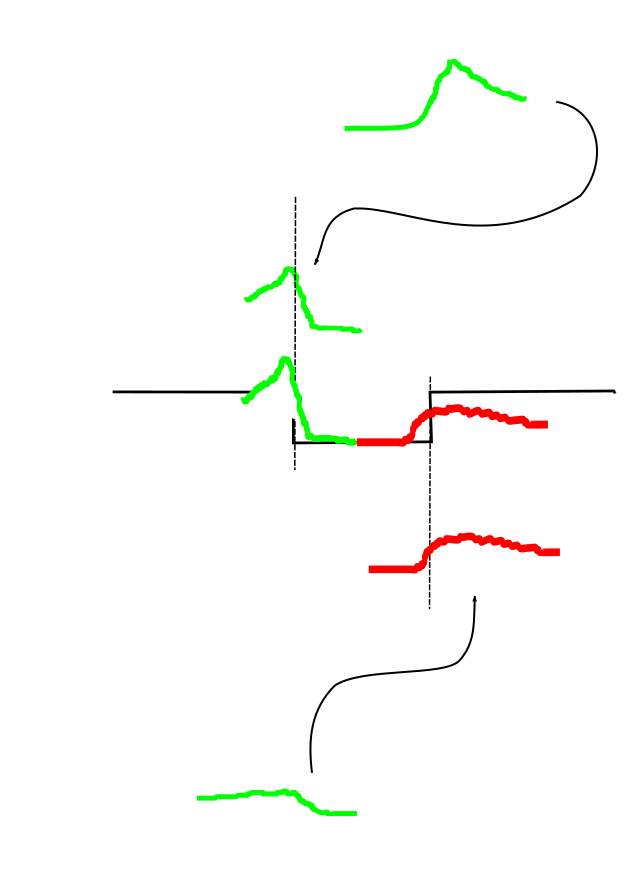
\includegraphics{TV_NotchDataConfig}}
  \caption[TV model optimisation configuration]{Expected mean rate response to notch noise in the TV cells is created from 1 octave notch sweeps (top) for the falling edge and from half octave notch sweeps (bottom) for the rising edge. (Top and bottom figures from Fig.~9 \citep*{ReissYoung:2005})}   \label{fig:TVNotchDiagram}
\end{figure}

% {
\small\linespread{0.5}
\begin{table}[htb]
    \caption{Tuberculoventral cell model summary}
    \label{tab:TVNotchModelSummary}
\end{table}
\noindent%
\begin{tabularx}{\textwidth}{|l|X|}\hline %
\hdr{2}{A}{Model Summary}\\\hline
         \textbf{Populations}          & HSR and LSR ANFs, Golgi, DS, and TV cells \\\hline
          \textbf{Topology}            & Tono-topicity of the rat AN and CN \\\hline
        \textbf{Connectivity}          & ANF$\to$\{GLG, DS, TV\}, GLG$\to$DS, DS$\to$TV  \\\hline
         \textbf{Input model}          & ANF~model: Instantaneous-rate Poisson neural model \citep{ZilanyBruce:2007} \\ \hline
\multirow{3}{*}{\textbf{Neuron model}} & GLG: Instantaneous-rate Poisson neural model\\
                                       & DS: HH-like single-compartment model (Type I-II \RM model)\\ 
                                       & TV: HH-like single-compartment model (Type I-classic \RM model) \\\hline
       \textbf{Channel models}         & $I_{\textrm{Na}}$, $I_{\textrm{KHT}}$, $I_{\textrm{KLT}}$, $I_{\textrm{KA}}$ and $I_{\textrm{h}}$ \citep{RothmanManis:2003b}\\\hline
\multirow{2}{*}{\textbf{Synapse model}} & Excitatory: AMPA glutamatergic receptor (single-exponential)\\
&  Inhibitory: \GABAa GABAergic receptor (double-exponential), Glycinergic receptor (double-exponential) \\\hline
%            \textbf{Input}             & Notch-noise stimulus \\\hline
%\textbf{Optimisation}    & Parameters for \GLGDS are optimised based on experimental click recovery date from \citet{BackoffPalombiEtAl:1997}. The praxis method is used for optimisation.  \\\hline
%\textbf{Measurements}    &  Spikes of TV units recorded and PSTH genereated. First spike latency, mean rate and variance of TV units calculated. Fitting data was compared against experimental data of a Type II~\DCN~unit~\citep[Figure~9]{ReissYoung:2005}.\\\hline
\end{tabularx}
\vspace{1ex}

% - B -----------------------------------------------------------------------------
\noindent%
\begin{tabularx}{\textwidth}{|l|X|X|}\hline
\hdr{3}{B}{Populations}\\\hline
\textbf{Name} &    \textbf{Elements}    & \textbf{Size} \\\hline
     HSR      &    Poisson generator    & $N_{\text{HSR}} = 50$ per freq.\ channel \\\hline
     LSR      &    Poisson generator    & $N_{\text{LSR}}= 30$  per freq.\ channel \\\hline
     GLG      &    Poisson generator    & $N_{\text{GLG}}= 1$  per freq.\ channel  \\\hline
     DS       &   Type I-II \RM model    & $N_{\text{DS}}= 1$ per freq.\ channel \\\hline
     TV       & Type I-classic \RM model & $N_{\text{TV}}= 1$ per freq.\ channel\\\hline
\end{tabularx}
\vspace{1ex}

% - C ------------------------------------------------------------------------------
\noindent%
\begin{tabularx}{\textwidth}{|l|l|l|X|}\hline
\hdr{4}{C}{Connectivity}\\\hline
\textbf{Name}  & \textbf{Source} & \textbf{Target} & \textbf{Pattern} \\\hline
%   ANF$\to$DS &       ANF       &   D~Stellate    & Skewed Gaussian, centered at CF, spread below CF \sANFDSl, spread above CF \sANFDSh \\\hline
    \ANFTV     &    LSR, HSR     &       TV        & 
Narrowband connection on CF, zero spread, weight \wLSRTV and \wHSRTV, number \nLSRTV and \nHSRTV, delay \dANFTV \\\hline
%   GLG$\to$DS &      Golgi      &   D~Stellate    & Gaussian, centered at CF with spread \sGLGDS \\\hline
    \DSTV      &       DS        &       TV        & 
Gaussian convergence, centered on CF, spread \protect{$\sigma^2 = \sGLGDS$}, weight \wGLGDS, number \nGLGDS, delay $\dGLGDS=0.5$ ms \\\hline
\multicolumn{4}{|>{\centering}X|}{\ANFGLG, \ANFDS, and \GLGDS from Table~\ref{tab:TVModelSummary} }\\\hline
\end{tabularx}
% , uniform weight \wANFDS for all synapses, number \nLSRDS \& \nHSRDS, delay \dANFDS
\vspace{1ex}

% - D ------------------------------------------------------------------------------
\noindent%
\begin{tabularx}{\textwidth}{|l|X|}\hline
\hdr{2}{D}{Neuron and Synapse Model}\\\hline
        \textbf{Name}          & TV cell model \\\hline
        \textbf{Type}          & Type I-classic \RM model \citep{RothmanManis:2003b}, conductance synapse input \\\hline
\textbf{Subthreshold dynamics} & Na, KHT, Ih, and leak currents \\\hline
       \textbf{Spiking}        & Emit spike when $v(t) \geq \theta$  \\\hline
\end{tabularx}
\vspace{1ex}
% \noindent\begin{tabularx}{\textwidth}{|p{0.150.95\textwidth}|X|}\hline
% \hdr{2}{D}{Neuron and Synapse Model}\\\hline
% \textbf{Name} &  \\\hline
% \textbf{Type} & \\\hline
% \raisebox{-4.5ex}{\parbox{0.95\textwidth}{\textbf{Subthreshold dynamics}}} &
% \rule{1em}{0em}\vspace*{-3.5ex}
%     \begin{equation*}
%       \begin{array}{r@{\;=\;}lll}
%       \tau \dot{V}(t) & -V(t) + R I(t) &\text{if} & t > t^*+\tau_{\text{rp}} \\
%       V(t) & V_{\text{r}} & \text{else} \\[2ex]
%       I(t) & \multicolumn{3}{l}{\frac{\tau}{R} \sum_{\tilde{t}} w
%         \delta(t-(\tilde{t}+\Delta))}
%       \end{array}
%     \end{equation*}
% \vspace*{-2.5ex}\rule{1em}{0em}
%  \\\hline
% \multirow{3}{*}{\textbf{Spiking}} &
%    If $V(t-)<\theta \wedge V(t+)\geq \theta$
% \vspace*{-1ex}
% \begin{enumerate}\setlength{\itemsep}{-0.5ex}
% \item set $t^* = t$
% \item emit spike with time-stamp $t^*$
% \end{enumerate}
% \vspace*{-4ex}\rule{1em}{0em}
% \\\hline
% \end{tabularx}
%\vspace{2ex}

\noindent%
\begin{tabularx}{\textwidth}{|l|X|}\hline %
\hdr{2}{E}{Optimisation}\\\hline
\textbf{Input Stimulus} & Notch-noise stimulus based on \citet{ReissYoung:2005}. Stop-band filtered white noise (60 dB SPL, 50 ms duration, 2 ms cosine squared on\slash off ramp, 20 ms delay), 30 dB half-octave stop-band width, centred on the middle of the network (5.8 kHz)\\\hline
%\multicolumn{2}{|c|}{\begin{minipage}[c]{0.8\textwidth} \includegraphics[width=0.8\textwidth,keepaspectratio]{./gfx/Notch-Wl-12.5kHz-0.5.eps} \end{minipage}}\\\hline
\textbf{Parameters} &     
\wHSRTV,
\wLSRTV,
\wDSTV, \nDSTV

\\\hline

    \textbf{Input}      & Stimulus induced Poisson spike trains from \GLG units, \HSR and \LSR\ \ANFs, and natural synaptic input from \DS units\\\hline
\textbf{Fitness Function} & Spiking output of all 100 TV units across the network recorded over 25 repetitions.\\
% %\multicolumn{2}{|c|}{\begin{minipage}[c]{0.8\textwidth} \includegraphics[width=0.8\textwidth,keepaspectratio]{./gfx/AN_rateplace_12.5_0.5.eps}\end{minipage}}\\\hline
%\textbf{Measurements}    & PSTH sampled at each click for 2 ms to measure click recovery\\\hline
% %\textbf{Optimisation}    & Parameters for \GLGDS are optimised based on experimental click recovery date from \citet{BackoffPalombiEtAl:1997}. The praxis method is used for optimisation.  \\\hline
    &  PSTH of TV cells, calculated for first spike latency and mean rate. Fitting data was compared against experimental data of a Type II \DCN unit \citep[Figure~9]{ReissYoung:2005}. \\\hline
\end{tabularx}
\vspace{1ex}

%  \textbf{Assumptions}    & The spread ANF to DS cells (\sANFDSh,\sANFDSl) is arbitrary at this point and will be explored in the next experiment.\\ \hline
%   \textbf{Function}     & Weighted mean squared error see listing below  \\ \hline


% % D~----------------------------------
% \begin{tabularx}{\linewidth}{|X|c|c|c|}
% \hdr{4}{F}{Optimisation} \\ \hline
%               \textbf{Parameters}                & \textbf{Name} & \textbf{Range} & \textbf{Best Values} \\\hline 
%         Weight of DS syn on TV  ($\mu$S)         &    \wDSTV     &  [1e-5,0.005]  & 0.0029 \\
%        Weight of ANF syn on TV  ($\mu$S)         &    \wANFTV    &  [1e-5,0.005]  & 0.00017 \\
%          Number of synapses, LSR to TV           &    \nLSRTV    &     [0,64]     & 8           \\
%          Number of synapses, HSR to TV           &    \nHSRTV    &     [0,64]     & 14          \\
% Spread of DS connections onto TV (channel units) &    \sDSTV     &     [0,10]     & 2.1         \\
% Offset of DS connections onto TV (channel units) &    \oDSTV     &     [0,10]     & 0.24        \\ \hline
% \end{tabularx}
}


%%% Local Variables: 
%%% mode: latex
%%% TeX-master: "SimpleResponses"
%%% TeX-PDF-mode: nil
%%% End: 



%%% Local Variables:
%%% mode: latex
%%% mode: tex-fold
%%% mode: visual-line
%%% TeX-master: "SimpleResponses"
%%% TeX-PDF-mode: nil
%%% End:
